\documentclass{ximera}  


%\usepackage{todonotes}
%\usepackage{mathtools} %% Required for wide table Curl and Greens
%\usepackage{cuted} %% Required for wide table Curl and Greens
\newcommand{\todo}{}

\usepackage{esint} % for \oiint
\ifxake%%https://math.meta.stackexchange.com/questions/9973/how-do-you-render-a-closed-surface-double-integral
\renewcommand{\oiint}{{\large\bigcirc}\kern-1.56em\iint}
\fi


\graphicspath{
  {./}
  {jpg}
  {ximeraTutorial/}
  {basicPhilosophy/}
  {functionsOfSeveralVariables/}
  {normalVectors/}
  {lagrangeMultipliers/}
  {vectorFields/}
  {greensTheorem/}
  {shapeOfThingsToCome/}
  {dotProducts/}
  {partialDerivativesAndTheGradientVector/}
  {../productAndQuotientRules/exercises/}
  {../motionAndPathsInSpace/exercises/}
  {../normalVectors/exercisesParametricPlots/}
  {../continuityOfFunctionsOfSeveralVariables/exercises/}
  {../partialDerivativesAndTheGradientVector/exercises/}
  {../directionalDerivativeAndChainRule/exercises/}
  {../commonCoordinates/exercisesCylindricalCoordinates/}
  {../commonCoordinates/exercisesSphericalCoordinates/}
  {../greensTheorem/exercisesCurlAndLineIntegrals/}
  {../greensTheorem/exercisesDivergenceAndLineIntegrals/}
  {../shapeOfThingsToCome/exercisesDivergenceTheorem/}
  {../greensTheorem/}
  {../shapeOfThingsToCome/}
  {../separableDifferentialEquations/exercises/}
  {vectorFields/}
}

\newcommand{\mooculus}{\textsf{\textbf{MOOC}\textnormal{\textsf{ULUS}}}}

\usepackage{tkz-euclide}\usepackage{tikz}
\usepackage{tikz-cd}
\usetikzlibrary{arrows}
\tikzset{>=stealth,commutative diagrams/.cd,
  arrow style=tikz,diagrams={>=stealth}} %% cool arrow head
\tikzset{shorten <>/.style={ shorten >=#1, shorten <=#1 } } %% allows shorter vectors

\usetikzlibrary{backgrounds} %% for boxes around graphs
\usetikzlibrary{shapes,positioning}  %% Clouds and stars
\usetikzlibrary{matrix} %% for matrix
\usepgfplotslibrary{polar} %% for polar plots
\usepgfplotslibrary{fillbetween} %% to shade area between curves in TikZ
\usetkzobj{all}
\usepackage[makeroom]{cancel} %% for strike outs
%\usepackage{mathtools} %% for pretty underbrace % Breaks Ximera
%\usepackage{multicol}
\usepackage{pgffor} %% required for integral for loops



%% http://tex.stackexchange.com/questions/66490/drawing-a-tikz-arc-specifying-the-center
%% Draws beach ball
\tikzset{pics/carc/.style args={#1:#2:#3}{code={\draw[pic actions] (#1:#3) arc(#1:#2:#3);}}}



\usepackage{array}
\setlength{\extrarowheight}{+.1cm}
\newdimen\digitwidth
\settowidth\digitwidth{9}
\def\divrule#1#2{
\noalign{\moveright#1\digitwidth
\vbox{\hrule width#2\digitwidth}}}





\newcommand{\RR}{\mathbb R}
\newcommand{\R}{\mathbb R}
\newcommand{\N}{\mathbb N}
\newcommand{\Z}{\mathbb Z}

\newcommand{\sagemath}{\textsf{SageMath}}


%\renewcommand{\d}{\,d\!}
\renewcommand{\d}{\mathop{}\!d}
\newcommand{\dd}[2][]{\frac{\d #1}{\d #2}}
\newcommand{\pp}[2][]{\frac{\partial #1}{\partial #2}}
\renewcommand{\l}{\ell}
\newcommand{\ddx}{\frac{d}{\d x}}

\newcommand{\zeroOverZero}{\ensuremath{\boldsymbol{\tfrac{0}{0}}}}
\newcommand{\inftyOverInfty}{\ensuremath{\boldsymbol{\tfrac{\infty}{\infty}}}}
\newcommand{\zeroOverInfty}{\ensuremath{\boldsymbol{\tfrac{0}{\infty}}}}
\newcommand{\zeroTimesInfty}{\ensuremath{\small\boldsymbol{0\cdot \infty}}}
\newcommand{\inftyMinusInfty}{\ensuremath{\small\boldsymbol{\infty - \infty}}}
\newcommand{\oneToInfty}{\ensuremath{\boldsymbol{1^\infty}}}
\newcommand{\zeroToZero}{\ensuremath{\boldsymbol{0^0}}}
\newcommand{\inftyToZero}{\ensuremath{\boldsymbol{\infty^0}}}



\newcommand{\numOverZero}{\ensuremath{\boldsymbol{\tfrac{\#}{0}}}}
\newcommand{\dfn}{\textbf}
%\newcommand{\unit}{\,\mathrm}
\newcommand{\unit}{\mathop{}\!\mathrm}
\newcommand{\eval}[1]{\bigg[ #1 \bigg]}
\newcommand{\seq}[1]{\left( #1 \right)}
\renewcommand{\epsilon}{\varepsilon}
\renewcommand{\phi}{\varphi}


\renewcommand{\iff}{\Leftrightarrow}

\DeclareMathOperator{\arccot}{arccot}
\DeclareMathOperator{\arcsec}{arcsec}
\DeclareMathOperator{\arccsc}{arccsc}
\DeclareMathOperator{\si}{Si}
\DeclareMathOperator{\scal}{scal}
\DeclareMathOperator{\sign}{sign}


%% \newcommand{\tightoverset}[2]{% for arrow vec
%%   \mathop{#2}\limits^{\vbox to -.5ex{\kern-0.75ex\hbox{$#1$}\vss}}}
\newcommand{\arrowvec}[1]{{\overset{\rightharpoonup}{#1}}}
%\renewcommand{\vec}[1]{\arrowvec{\mathbf{#1}}}
\renewcommand{\vec}[1]{{\overset{\boldsymbol{\rightharpoonup}}{\mathbf{#1}}}\hspace{0in}}

\newcommand{\point}[1]{\left(#1\right)} %this allows \vector{ to be changed to \vector{ with a quick find and replace
\newcommand{\pt}[1]{\mathbf{#1}} %this allows \vec{ to be changed to \vec{ with a quick find and replace
\newcommand{\Lim}[2]{\lim_{\point{#1} \to \point{#2}}} %Bart, I changed this to point since I want to use it.  It runs through both of the exercise and exerciseE files in limits section, which is why it was in each document to start with.

\DeclareMathOperator{\proj}{\mathbf{proj}}
\newcommand{\veci}{{\boldsymbol{\hat{\imath}}}}
\newcommand{\vecj}{{\boldsymbol{\hat{\jmath}}}}
\newcommand{\veck}{{\boldsymbol{\hat{k}}}}
\newcommand{\vecl}{\vec{\boldsymbol{\l}}}
\newcommand{\uvec}[1]{\mathbf{\hat{#1}}}
\newcommand{\utan}{\mathbf{\hat{t}}}
\newcommand{\unormal}{\mathbf{\hat{n}}}
\newcommand{\ubinormal}{\mathbf{\hat{b}}}

\newcommand{\dotp}{\bullet}
\newcommand{\cross}{\boldsymbol\times}
\newcommand{\grad}{\boldsymbol\nabla}
\newcommand{\divergence}{\grad\dotp}
\newcommand{\curl}{\grad\cross}
%\DeclareMathOperator{\divergence}{divergence}
%\DeclareMathOperator{\curl}[1]{\grad\cross #1}
\newcommand{\lto}{\mathop{\longrightarrow\,}\limits}

\renewcommand{\bar}{\overline}

\colorlet{textColor}{black}
\colorlet{background}{white}
\colorlet{penColor}{blue!50!black} % Color of a curve in a plot
\colorlet{penColor2}{red!50!black}% Color of a curve in a plot
\colorlet{penColor3}{red!50!blue} % Color of a curve in a plot
\colorlet{penColor4}{green!50!black} % Color of a curve in a plot
\colorlet{penColor5}{orange!80!black} % Color of a curve in a plot
\colorlet{penColor6}{yellow!70!black} % Color of a curve in a plot
\colorlet{fill1}{penColor!20} % Color of fill in a plot
\colorlet{fill2}{penColor2!20} % Color of fill in a plot
\colorlet{fillp}{fill1} % Color of positive area
\colorlet{filln}{penColor2!20} % Color of negative area
\colorlet{fill3}{penColor3!20} % Fill
\colorlet{fill4}{penColor4!20} % Fill
\colorlet{fill5}{penColor5!20} % Fill
\colorlet{gridColor}{gray!50} % Color of grid in a plot

\newcommand{\surfaceColor}{violet}
\newcommand{\surfaceColorTwo}{redyellow}
\newcommand{\sliceColor}{greenyellow}




\pgfmathdeclarefunction{gauss}{2}{% gives gaussian
  \pgfmathparse{1/(#2*sqrt(2*pi))*exp(-((x-#1)^2)/(2*#2^2))}%
}


%%%%%%%%%%%%%
%% Vectors
%%%%%%%%%%%%%

%% Simple horiz vectors
\renewcommand{\vector}[1]{\left\langle #1\right\rangle}


%% %% Complex Horiz Vectors with angle brackets
%% \makeatletter
%% \renewcommand{\vector}[2][ , ]{\left\langle%
%%   \def\nextitem{\def\nextitem{#1}}%
%%   \@for \el:=#2\do{\nextitem\el}\right\rangle%
%% }
%% \makeatother

%% %% Vertical Vectors
%% \def\vector#1{\begin{bmatrix}\vecListA#1,,\end{bmatrix}}
%% \def\vecListA#1,{\if,#1,\else #1\cr \expandafter \vecListA \fi}

%%%%%%%%%%%%%
%% End of vectors
%%%%%%%%%%%%%

%\newcommand{\fullwidth}{}
%\newcommand{\normalwidth}{}



%% makes a snazzy t-chart for evaluating functions
%\newenvironment{tchart}{\rowcolors{2}{}{background!90!textColor}\array}{\endarray}

%%This is to help with formatting on future title pages.
\newenvironment{sectionOutcomes}{}{}



%% Flowchart stuff
%\tikzstyle{startstop} = [rectangle, rounded corners, minimum width=3cm, minimum height=1cm,text centered, draw=black]
%\tikzstyle{question} = [rectangle, minimum width=3cm, minimum height=1cm, text centered, draw=black]
%\tikzstyle{decision} = [trapezium, trapezium left angle=70, trapezium right angle=110, minimum width=3cm, minimum height=1cm, text centered, draw=black]
%\tikzstyle{question} = [rectangle, rounded corners, minimum width=3cm, minimum height=1cm,text centered, draw=black]
%\tikzstyle{process} = [rectangle, minimum width=3cm, minimum height=1cm, text centered, draw=black]
%\tikzstyle{decision} = [trapezium, trapezium left angle=70, trapezium right angle=110, minimum width=3cm, minimum height=1cm, text centered, draw=black]




 
\title{Magnetic Coupling} 
\author{Milica Markovic} 
\outcome{Apply Faraday's Law to circuits.}
\begin{document}  
\begin{abstract}  

\end{abstract}  
\maketitle    


\section{Applications of Faraday's law to AC circuits}


We will now look at an example of two coils carrying alternating current, as shown in Figure \ref{fig:CoupledCoilsAC}. The coils are connected to two AC signal generators, and have internal resistance R. 

\begin{figure}[htbp]
\begin{center}
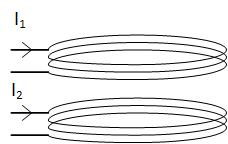
\includegraphics[scale=0.7]{../jpg/coupledCoils.jpg}
\end{center}
\caption{}
\label{fig:CoupledCoilsAC}
\end{figure}

\subsection{Coils with no coupling}

We will first look at the case when the coils are not coupled. We will see that these are two simple RL circuits.
If the coils are not coupled, the mutual flux is zero, and the fluxes through the coils are

\begin{eqnarray}
\Phi_{1s}= L_1 I_1 \\
\Phi_{2s}= L_2 I_2
\end{eqnarray}

The above equation states that the currents in the coils are in phase with flux $\Phi$. This equation is similar to two other equations that define resistance and capacitance. V=R I  means that the current is in phase with the voltage on a resistor. Q=C V, the charge is in phase with the voltage on a capacitor. 

Since mutual flux is zero, according to Faraday's law, the induced voltage in each coil is

\begin{eqnarray}
e_1=-\frac{d\Phi_{1s}}{dt} = - L_1 \frac{dI_1}{dt}\\
e_2=-\frac{d\Phi_{2s}}{dt} = - L_2 \frac{dI_2}{dt}
\end{eqnarray}

The induced voltage and the voltage in the rest of the circuit are related through Faraday's law:

\begin{equation}
\oint_c \vec{E} \cdot \vec{dl} =  - \frac{d\Phi}{dt}
\end{equation}

Induced current flows as a current would inside the generator, from negative to positive voltage terminal, as shown in Figure \ref{fig:InducedEMF}.



\begin{figure}[htbp]
\begin{center}
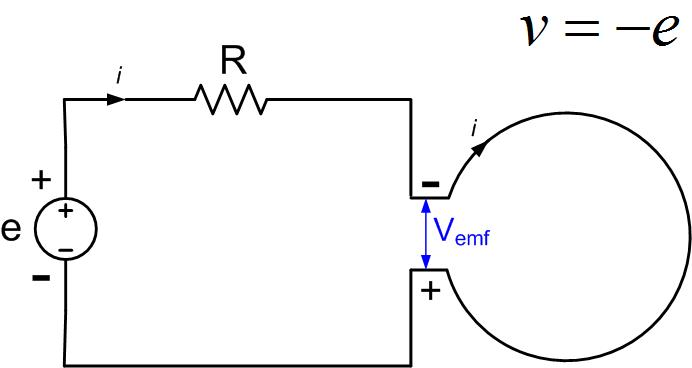
\includegraphics[scale=0.5]{../jpg/Loop_Inductance.jpg}
\end{center}
\caption{Voltage at the end of the coil and the induced emf.}
\label{fig:InducedEMF}
\end{figure}


 Therefore,
the voltage at the output of the coils is $v_1=-e_1$ and $v_2=-e_2$

\begin{eqnarray}
v_1= L_1 \frac{dI_1}{dt} \\
v_2= L_2 \frac{dI_2}{dt}
\end{eqnarray}



The above equation states that the voltage at the coils' output leads the current and flux, by $90^0$, if we assume that the resistance in Figure \ref{fig:InducedEMF} is small.


 If the resistance is not small, then the voltage will be leading with angle $\arctan(\frac{\omega L}{R})$. We can derive this equation from Faraday's law.
 
 

\begin{equation}
\oint_c \vec{E} \cdot \vec{dl} =  - \frac{d\Phi}{dt}
\end{equation}

If we integrate the electric field along the closed loop and assume that the resistance of the coil and other losses are included in R

\begin{eqnarray}
-e + R I = - L \frac{d I}{dt}
\end{eqnarray}

We see that this is a time-domain equation for an RL circuit. If we use the definition of phasors, we get 

\begin{eqnarray}
\tilde{E} = (R + j \omega L) \tilde{I}
\end{eqnarray}

Therefore the voltage will be leading current by an angle $\arctan(\frac{\omega L}{R})$.

\subsection{Coils with coupling}

When two coils are close together, their magnetic fields couple and some of the flux from coil 1 will pass through the second coil. This additional flux produces induced voltage in the second coil, as we discussed before. The amount of interaction between the coils is called mutual flux. Associated with mutual flux is mutual inductance $M=L_{12}=\frac{\Phi_{1}}{I_2}=L_{21}=\frac{\Phi_{2}}{I_1}	$. Mutual inductance can be positive or negative, as we have seen before because the fluxes can add or subtract. The mutual flux through coil 1 can be in phase or out of phase with the current that produced it.

If the coils are coupled, the mutual flux is not zero, and the fluxes through the coils are

\begin{eqnarray}
\Phi_1=\Phi_{1s} + \Phi_{21} = L_{1s} I_1 \pm L_{12} I_2 \\
\Phi_2= \Phi_{2s} + \Phi_{12} = L_{2s} I_2 \pm L_{21} I_1 
\end{eqnarray}

The induced voltages in each coil are


\begin{eqnarray}
e_1=  -L_1 \frac{dI_1}{dt} \mp L_{12} \frac{dI_2}{dt} \\
e_2= - L_2 \frac{dI_2}{dt} \mp L_{21} \frac{dI_1}{dt}
\end{eqnarray}

The voltages at the end of the coils are therefore


\begin{eqnarray}
v_1=  L_1 \frac{dI_1}{dt} \pm L_{12} \frac{dI_2}{dt} \\
v_2= L_2 \frac{dI_2}{dt} \pm L_{21} \frac{dI_1}{dt}
\end{eqnarray}


It is difficult in circuit notation to describe how fluxes are adding or subtracting. Therefore a "dot" notation is developed to explain flux interaction on a circuit diagram. For example, in Figure \ref{fig:DotNotation1}, two coupled coils connected in series are shown. If the current flows from left (or right), it will encounter a dot (or no dot) at each inductor. The fluxes will therefore add, and the equations that we write are

 
\begin{figure}[htbp]
\begin{center}
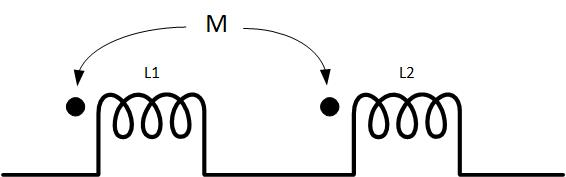
\includegraphics[scale=0.8]{../jpg/CoupledCoilsCircuit.jpg}
\end{center}
\caption{Dot notation.}
\label{fig:DotNotation1}
\end{figure}





\begin{eqnarray}
v_1=  L_1 \frac{dI}{dt} + L_{12} \frac{dI}{dt} \\
v_2= L_2 \frac{dI}{dt} + L_{21} \frac{dI}{dt}
\end{eqnarray}

The above equations show that the self and mutual inductance add.


\begin{eqnarray}
v_1=  (L_1  + L_{12}) \frac{dI}{dt} \\
v_2= (L_2 + L_{21}) \frac{dI}{dt}
\end{eqnarray}


Figure \ref{fig:DotNotation2} shows two coupled coils connected in series, but this time the dots are on the opposite sides of the coils. If the current flows from the left, it will encounter a dot at the first inductor but no dot on the second inductor. The fluxes will  therefore subtract, the mutual inductance is negative, and the equations that we write are

 


\begin{figure}[htbp]
\begin{center}
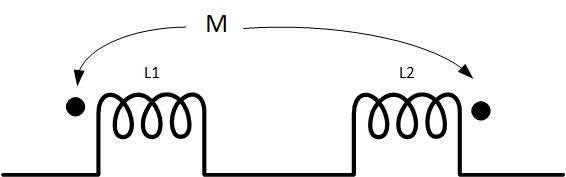
\includegraphics[scale=0.8]{../jpg/CoupledCoilsCircuit2.jpg}
\end{center}
\caption{Dot notation.}
\label{fig:DotNotation2}
\end{figure}

\begin{eqnarray}
v_1=  L_1 \frac{dI}{dt} - L_{12} \frac{dI}{dt} \\
v_2= L_2 \frac{dI}{dt} - L_{21} \frac{dI}{dt}
\end{eqnarray}


Or

\begin{eqnarray}
v_1=  (L_1  - L_{12}) \frac{dI}{dt} \\
v_2= (L_2 - L_{21}) \frac{dI}{dt}
\end{eqnarray}




The above equations show that the self and mutual inductance subtract.



In phasor notation and a circuit like the one in Figure \ref{fig:InducedEMF}, the only difference is the addition of the mutual inductance. So the equations will be



\begin{eqnarray}
\tilde{E_1} = (R + j \omega L_1) \tilde{I_1} \pm j \omega L_{12} I_2 \\
\tilde{E_1} = (R + j \omega L_2) \tilde{I_2} \pm j \omega L_{21} I_1 
\end{eqnarray}





\end{document} 

